\section{Theory}
\label{section: Chapter4/theory}

In Chapter \ref{section: Chapter3}, the mathematical model for single-phase fluid-driven fracture is described in Section \ref{formulation}. In what follows, this same model is assumed, as all derivations are independent of the system dimensionality as well as fracture shapes. More precisely, since the multi-resolution framework will be used, two coexisting descriptions are used. In a global domain, cracks are assumed to be represented by two-dimensional surfaces embedded in the 3D domain and the governing equations and boundary condition are those from \eqref{linear momentum balance} - \eqref{pf_ic}, which assume a fixed fracture geometry. In the local domain, which will be described next, the fracture problem is treated with a variational phase-field formulation, given by \eqref{basic u problem}-\eqref{eq:ddot-strong} which assume flow quantities to be fixed.

A more detailed discussion of the motivation and fundamentals of the multi-resolution method is provided in Section \ref{numerics}. In a nutshell, it breaks a fracture problem in two separate problems. In the global one, that covers the whole domain, a discrete representation of the fracture is used, but its geometry is assumed to be fixed. To account for crack propagation, a local problem in a vicinity of the fracture front is set up, employing the phase-field method, taking advantage of its flexibility in representing evolving fracture geometries.

This type approach is particularly interesting for simulating fluid-driven fracture due to the presence of a discrete fracture in the global level, which simplifies the computation of the fracture apertures that must be coupled to the fluid problem. If a pure phase-field description is used, extracting these apertures becomes a challenging task. In addition to that, a multi-resolution approach can also alleviate the computational cost that comes with the high-refined grids needed to solve phase-field problems. This becomes a remarkable limitation in the context of hydraulic fracturing since the length of fractures is usually of the order of kilometers.

An attentive reader will realize that the multi-resolution algorithm proposed in Chapter \ref{section: Chapter3} is not easily extendable to three-dimensions only because of the propagation step described in the subsection \ref{propagation_step}. In this part of the algorithm, a crack tip location is extracted from the damage field in the local problem and used to inform the global problem how to advance the crack. The concept of a crack tip does not exist in three-dimensions (it becomes a fracture front). In addition to that, while in 2D it is possible to connect line cuts (which are just line segments) to form an approximation to the crack geometry, in 3D these become planar cuts, which may fail to connect on element boundaries. SHOW FIGURE. 

The first extension discussed in this chapter deals with the case of planar fractures in 3D. The main challenge here consists of tracking the entire fracture front and evolving it according to the damage field computed in the local problem. This is done defining a discrete set of crack front elements which are investigated for damage throughout the problem execution. The construction of this layer of front elements ahead of the crack prevents is important to preserve the accuracy of the solution, because the lack fluid flow in the local problem can lead to spurious unstable solutions.

For the more complex case of non-planar fracture propagation, some considerations will be discussed in section \ref{}. The prototype of an algorithm to handle this case will be shown together with some preliminary results. However, it's robustness is not guaranteed. 

algorithm summary and figures

some results xda

\begin{figure}[h]
    \centering
    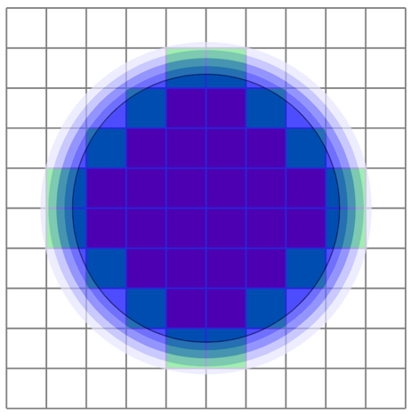
\includegraphics[width=0.5\linewidth]{Chapter4/figures/blue_circle.png}
    \caption{Multi-resolution solution algorithm.}
    \label{fig:lorem1}
\end{figure}


\begin{figure}[h]
    \centering
    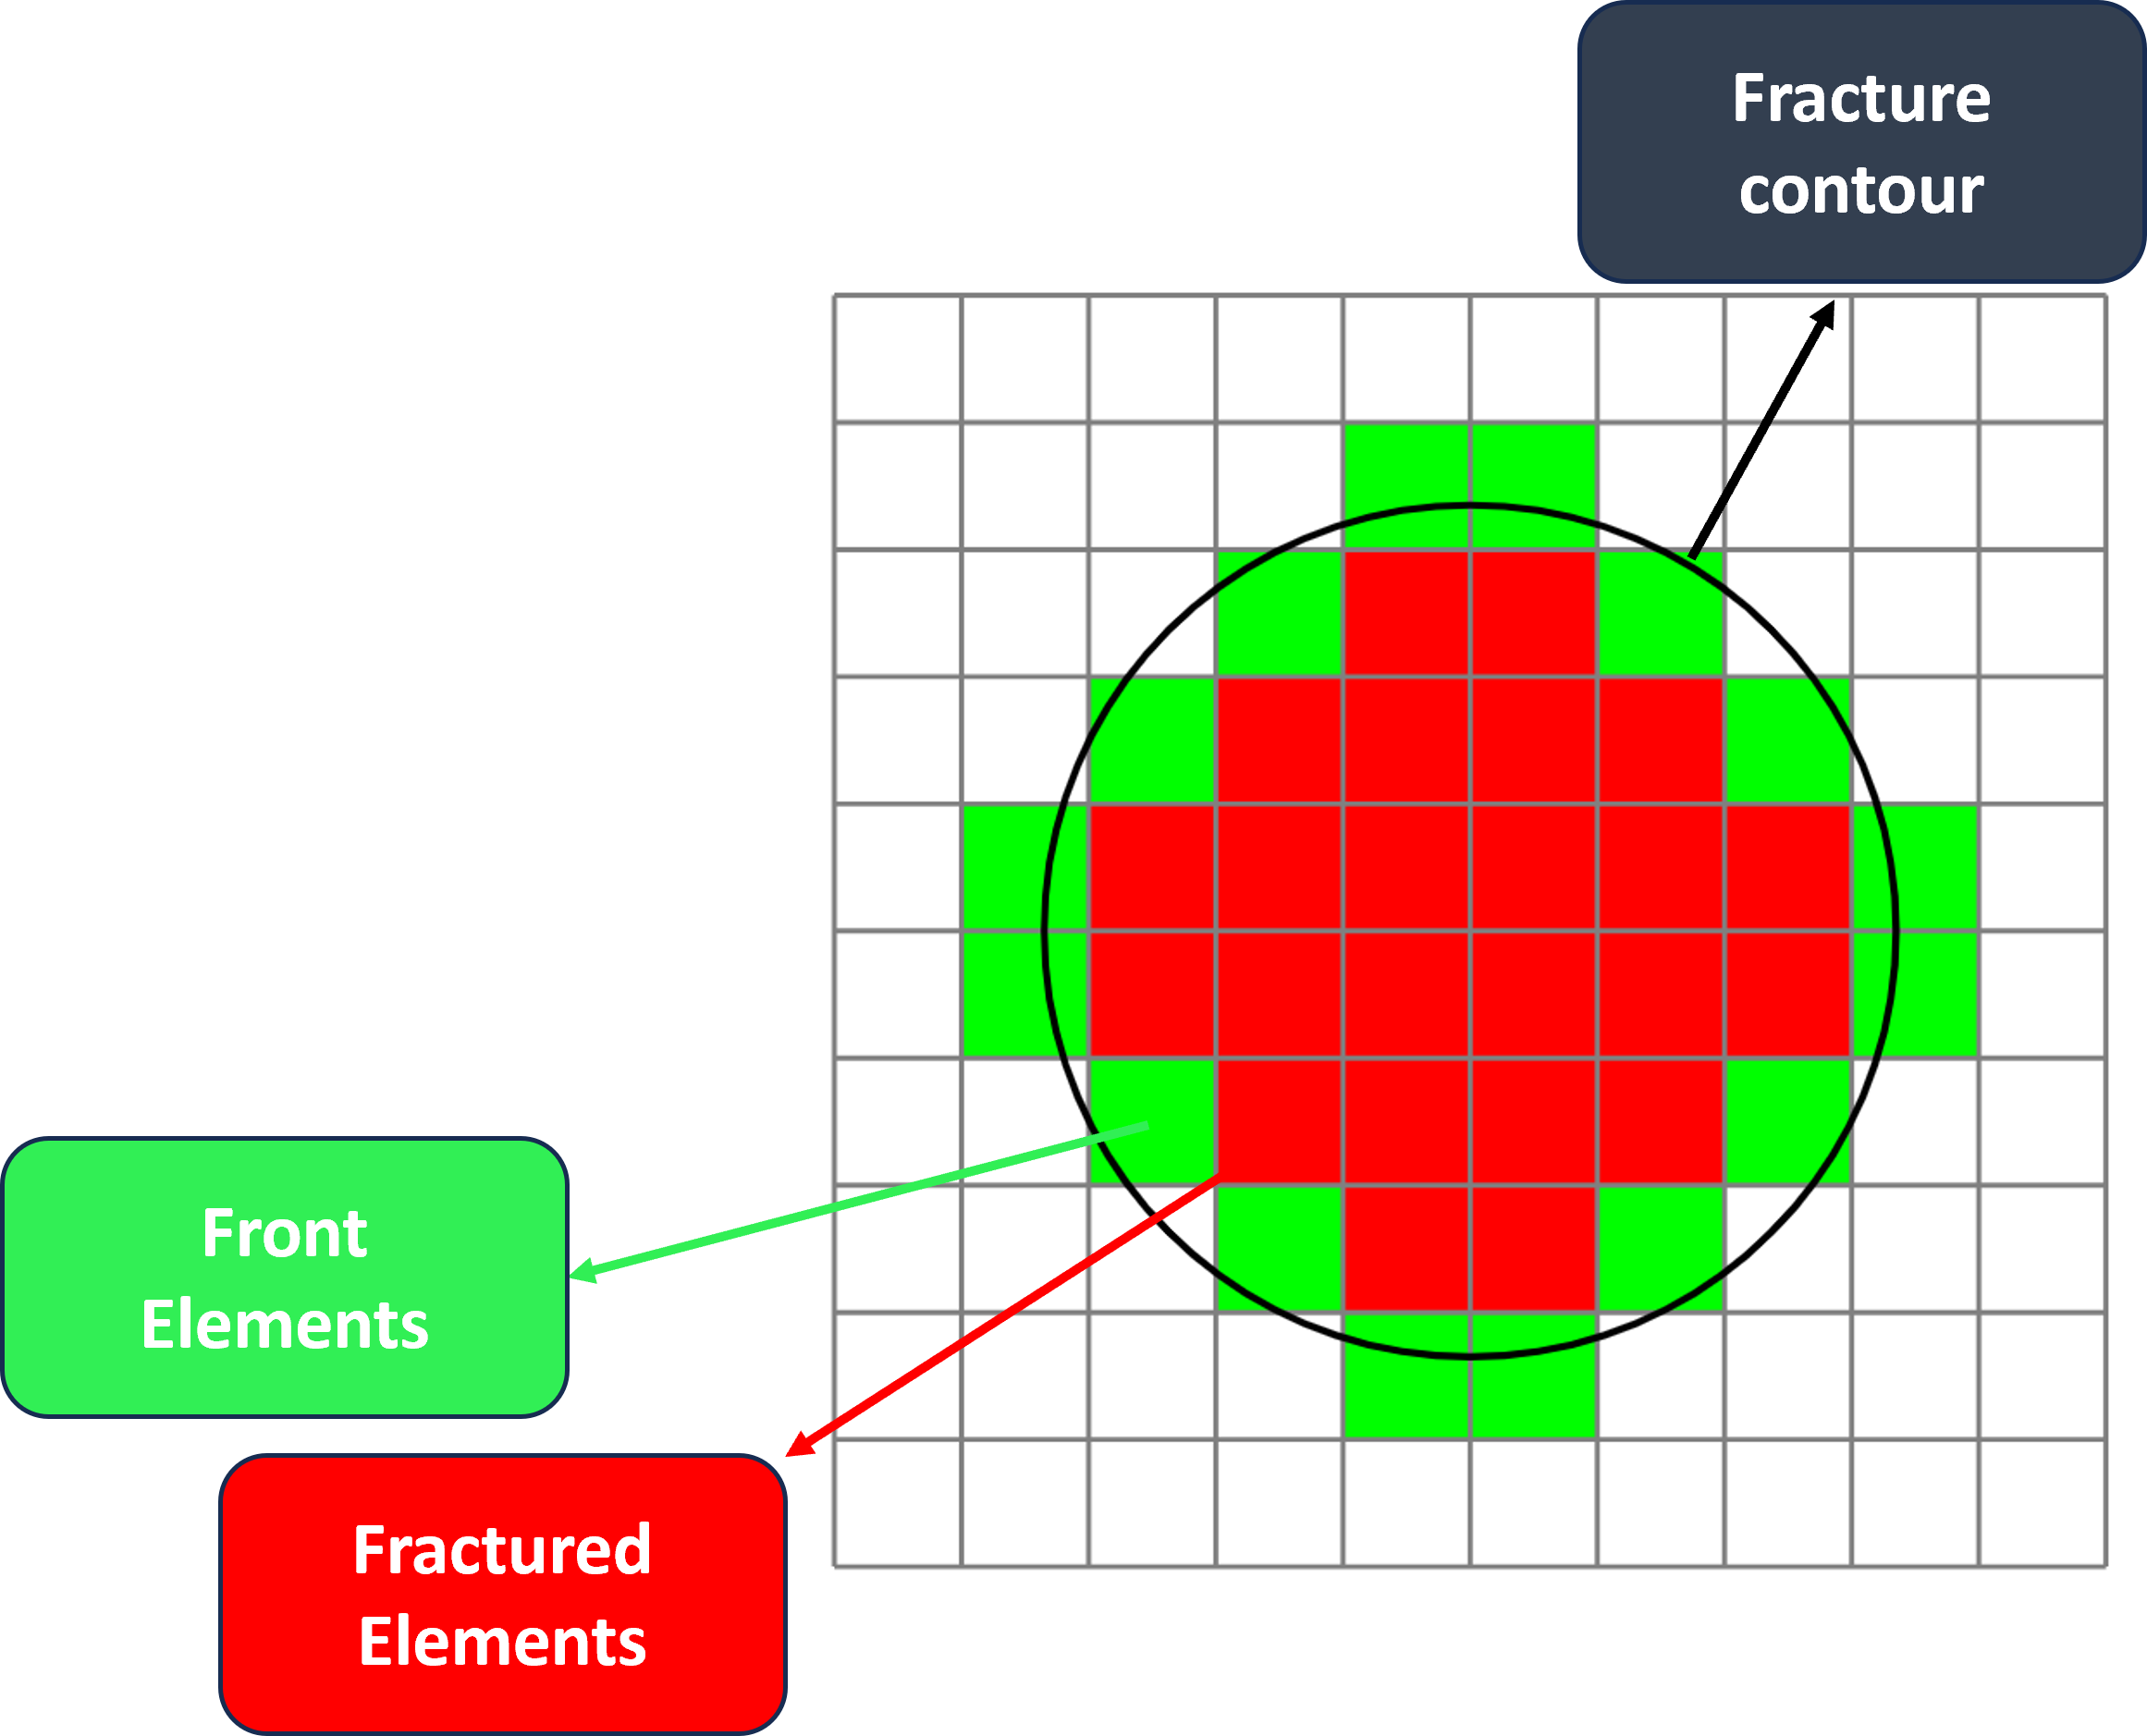
\includegraphics[width=\linewidth]{Chapter4/figures/penny_with_descriptions.png}
    \caption{Multi-resolution solution algorithm.}
    \label{fig:lorem4}
\end{figure}

\begin{figure}[h]
    \centering
    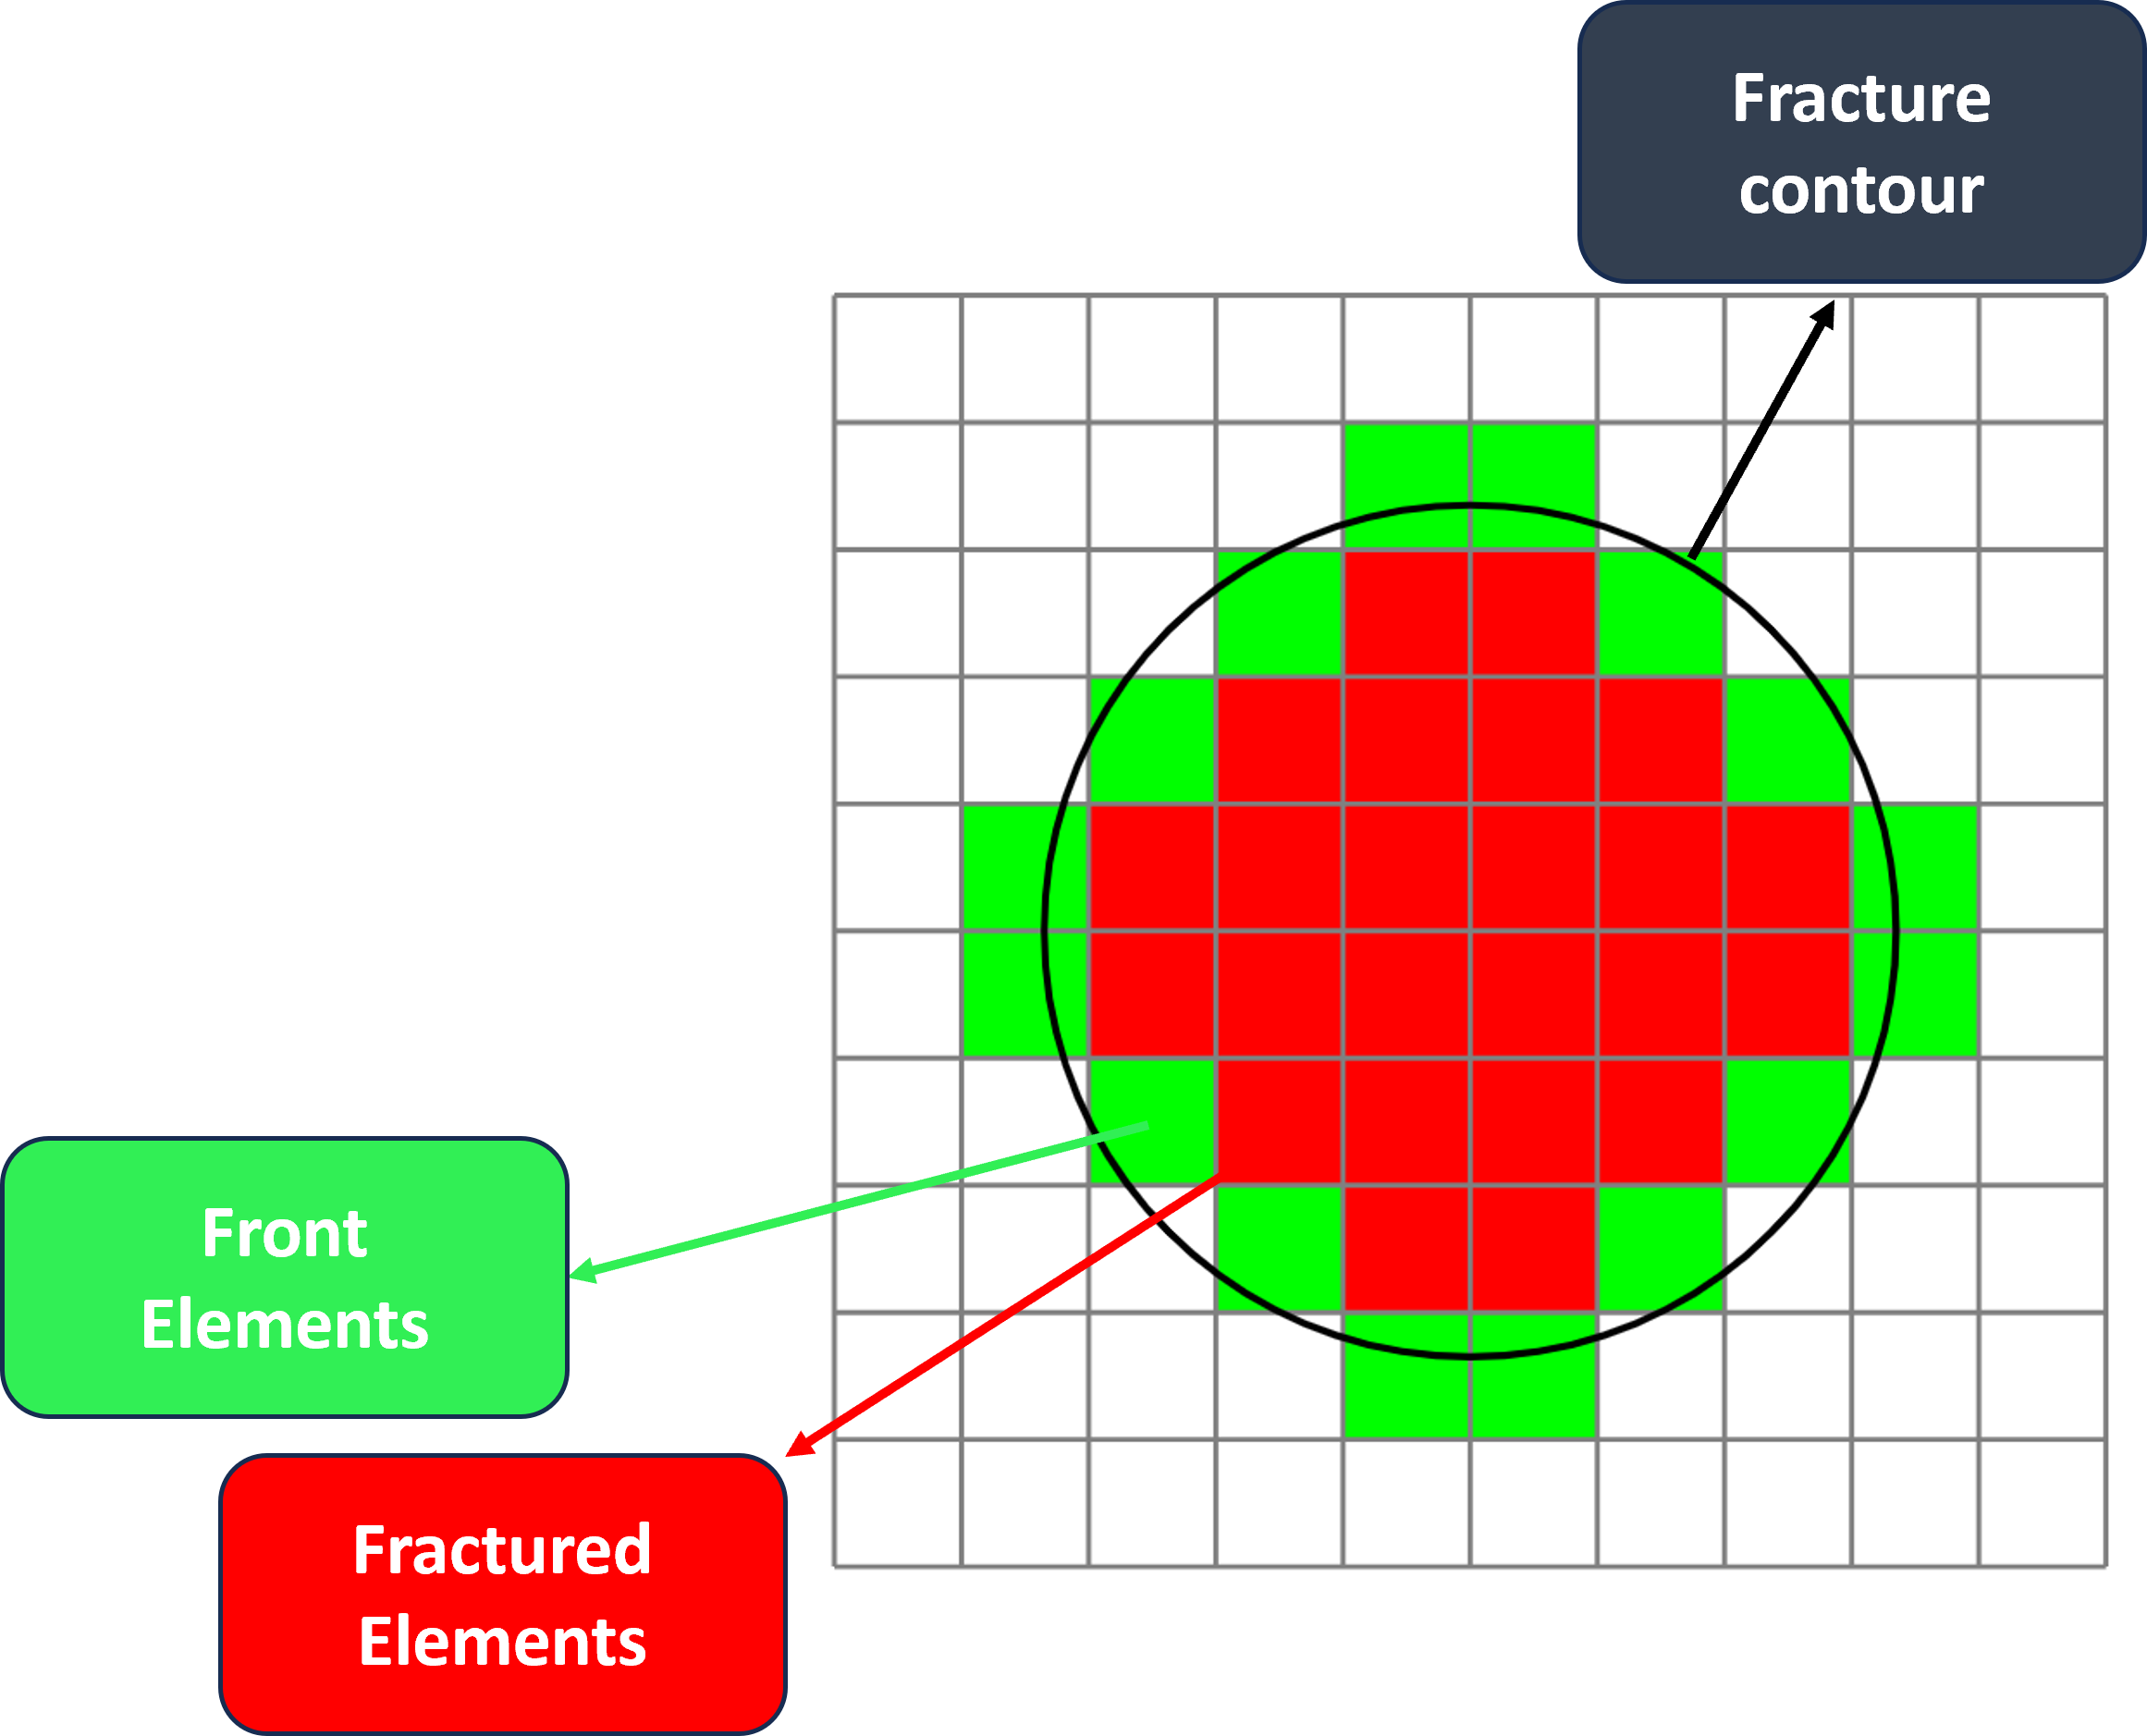
\includegraphics[width=\linewidth]{Chapter4/figures/penny_with_descriptions.png}
    \caption{Multi-resolution solution algorithm.}
    \label{fig:lorem4}
\end{figure}

\begin{figure}[h]
    \centering
    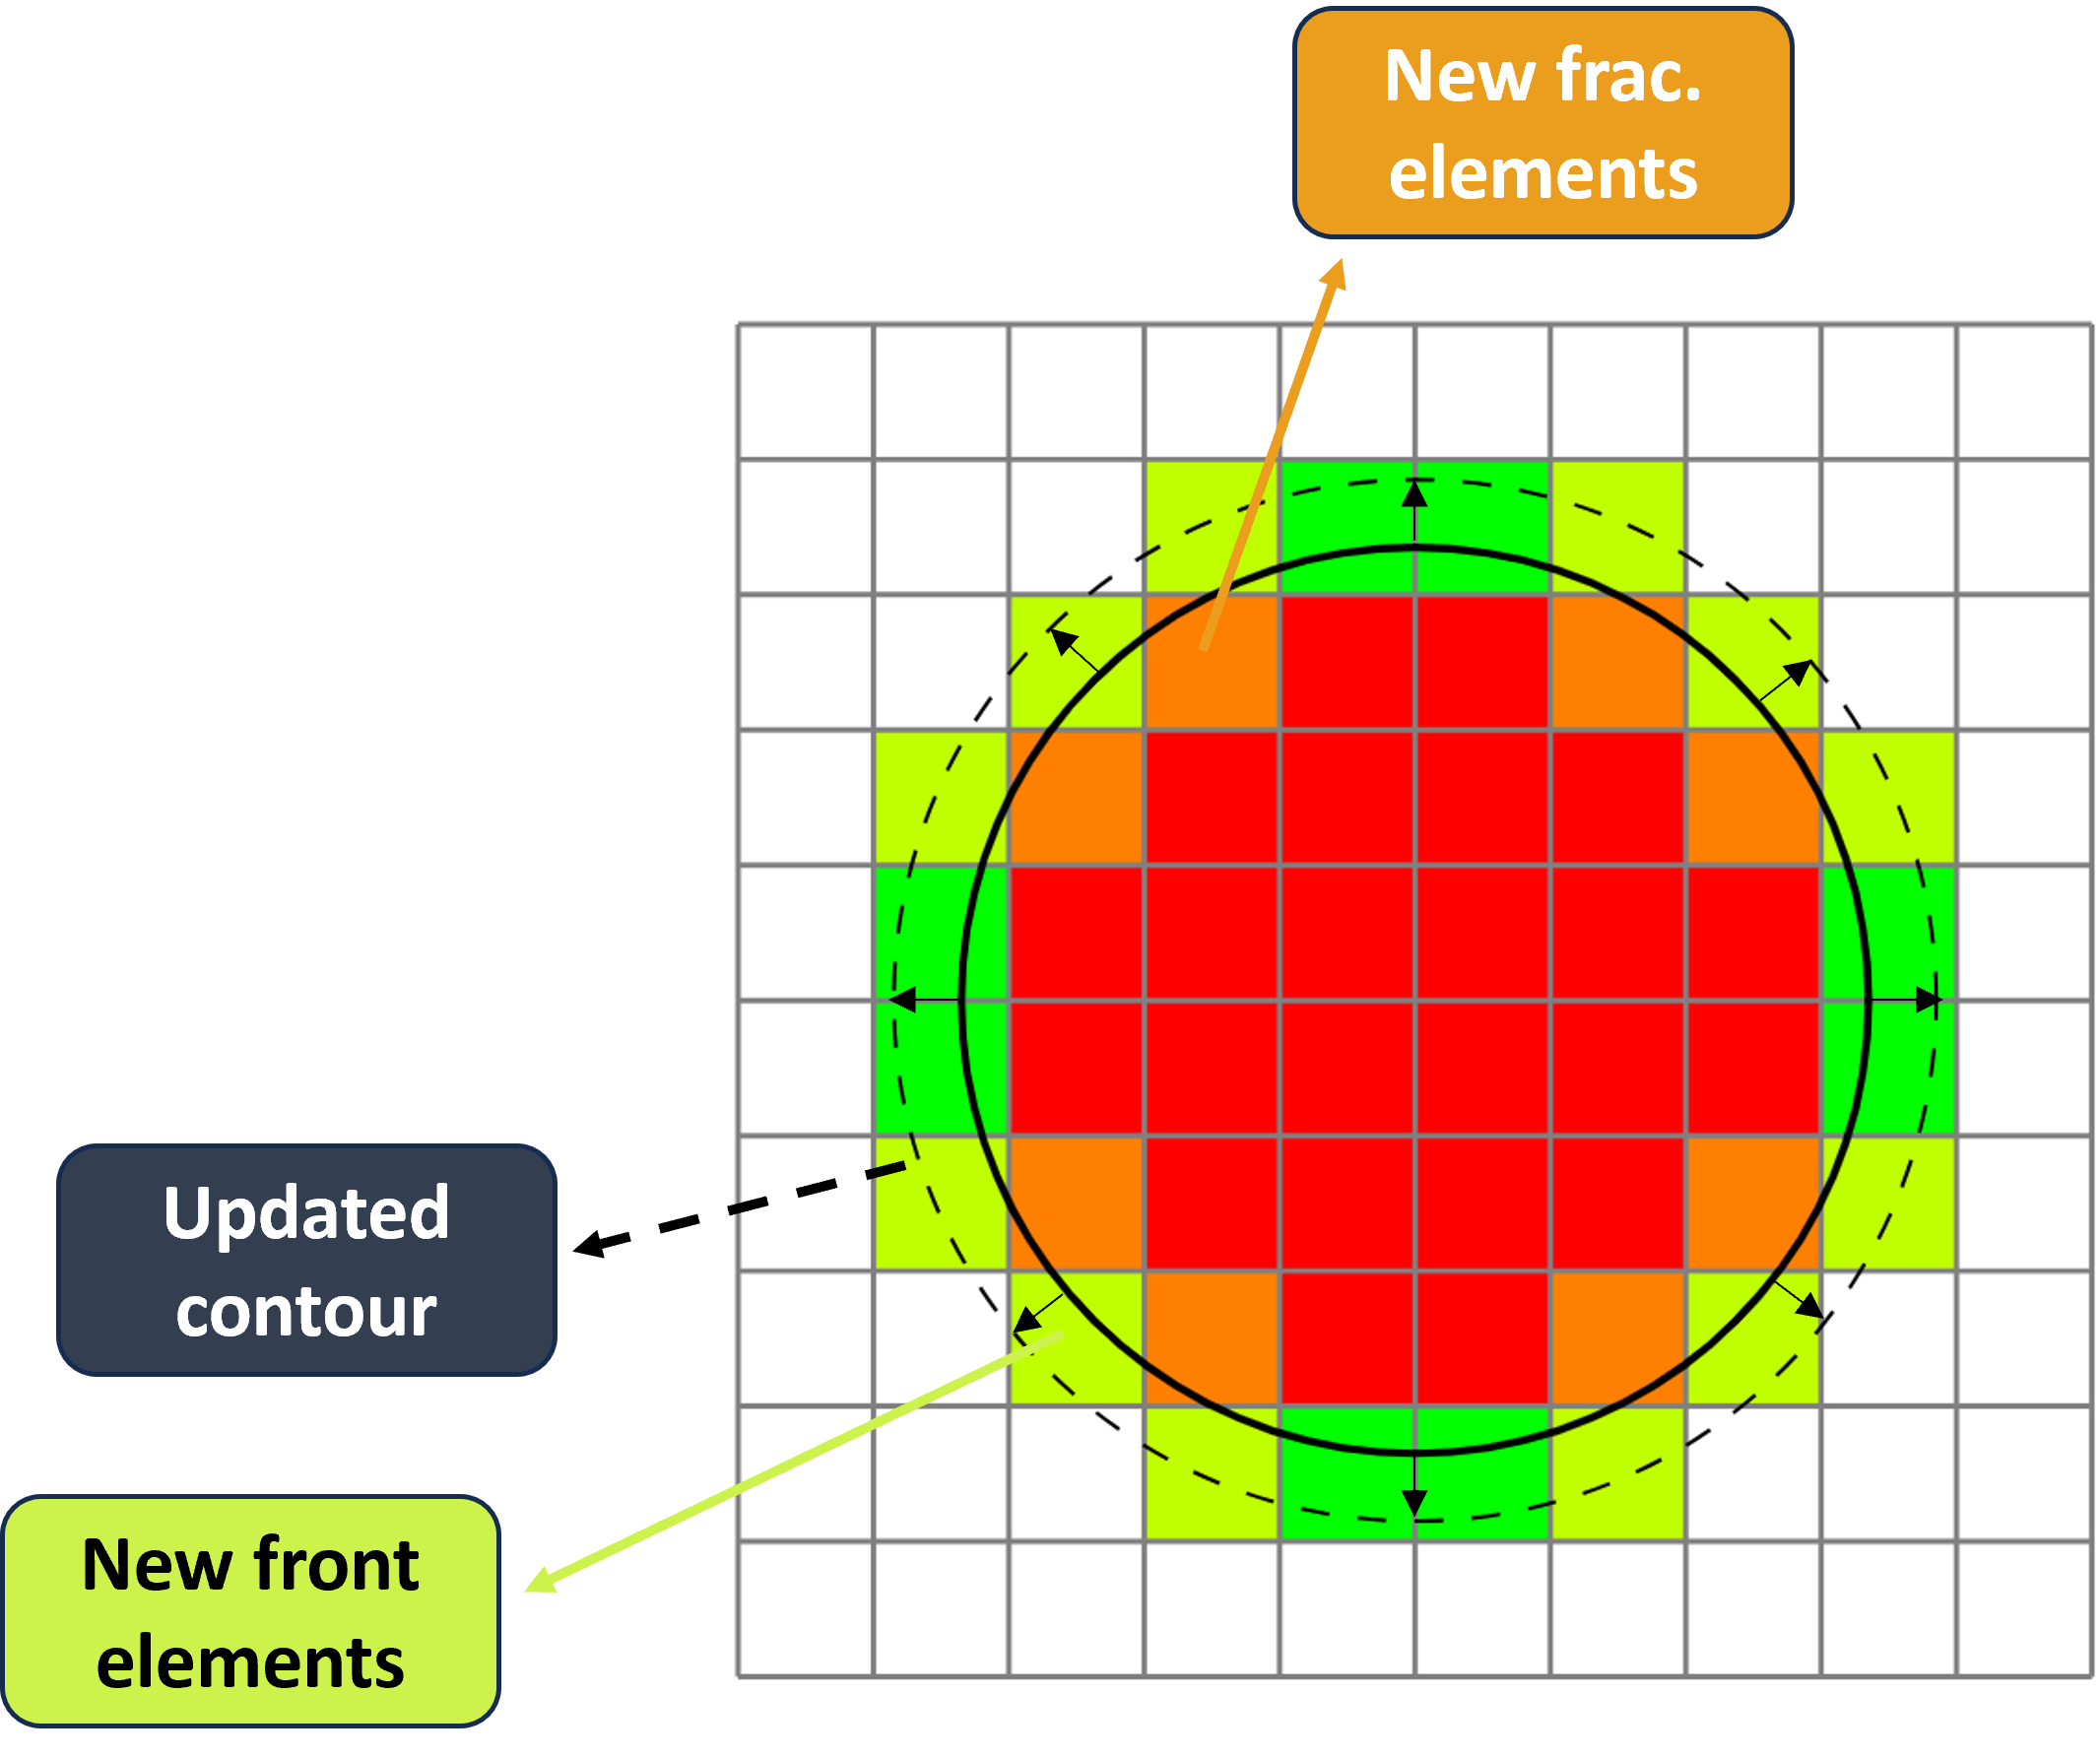
\includegraphics[width=\linewidth]{Chapter4/figures/larger_penny_with_descriptions.png}
    \caption{Multi-resolution solution algorithm.}
    \label{fig:lorem2}
\end{figure}

\begin{figure}[h]
    \centering
    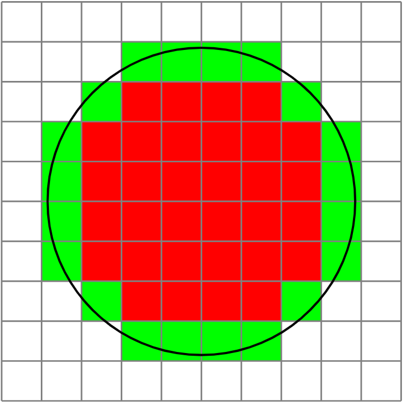
\includegraphics[width=0.5\linewidth]{Chapter4/figures/larger_penny.png}
    \caption{Multi-resolution solution algorithm.}
    \label{fig:lorem3}
\end{figure}

\begin{figure}[h]
    \centering
    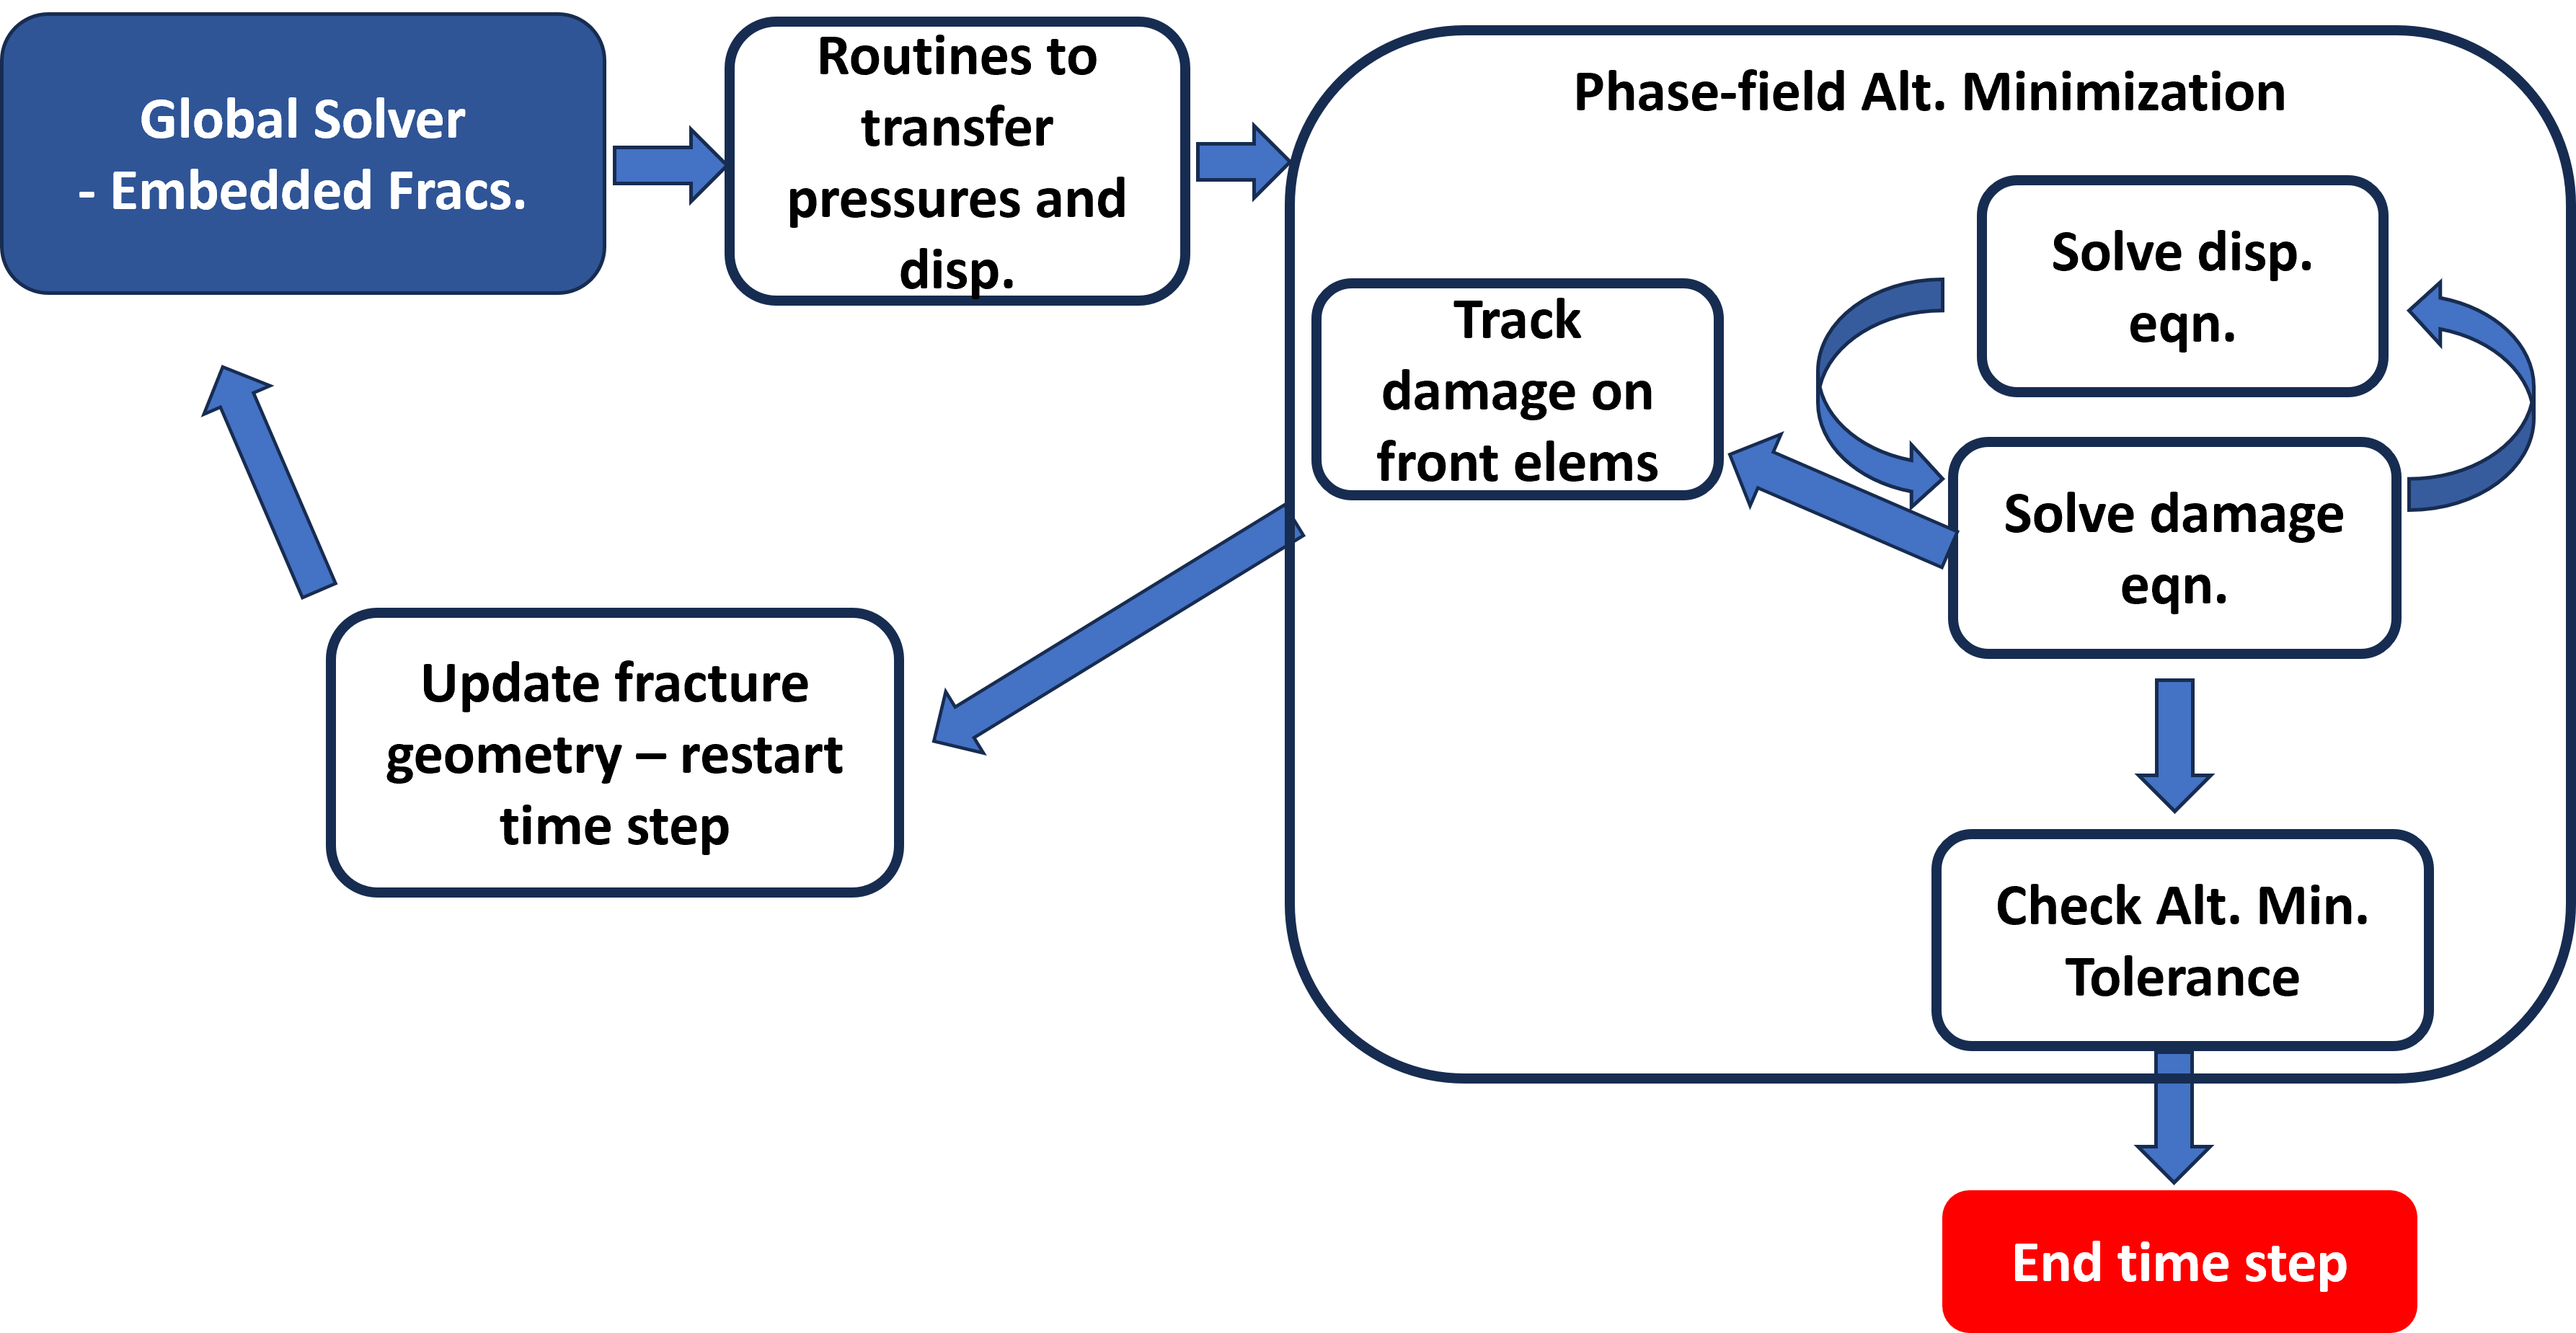
\includegraphics[width=\linewidth]{Chapter4/figures/planar3D_algorithm.png}
    \caption{Multi-resolution solution algorithm.}
    \label{fig:lorem5}
\end{figure}
